\documentclass[11pt]{article}
\usepackage{amssymb}
\usepackage{amsmath}
\usepackage{graphicx}
\usepackage{fullpage}
\usepackage{gensymb}
\usepackage{float}
\usepackage{upgreek}
\usepackage{hyperref}
\graphicspath{ {C:\Users\Dat\Documents\GitHub\Arduino\exp11-night-light} }
\usepackage[margin=2cm]{geometry}
\tolerance=1000
\date{}
\title{Night Light}
\begin{document}
\maketitle

\centerline{
	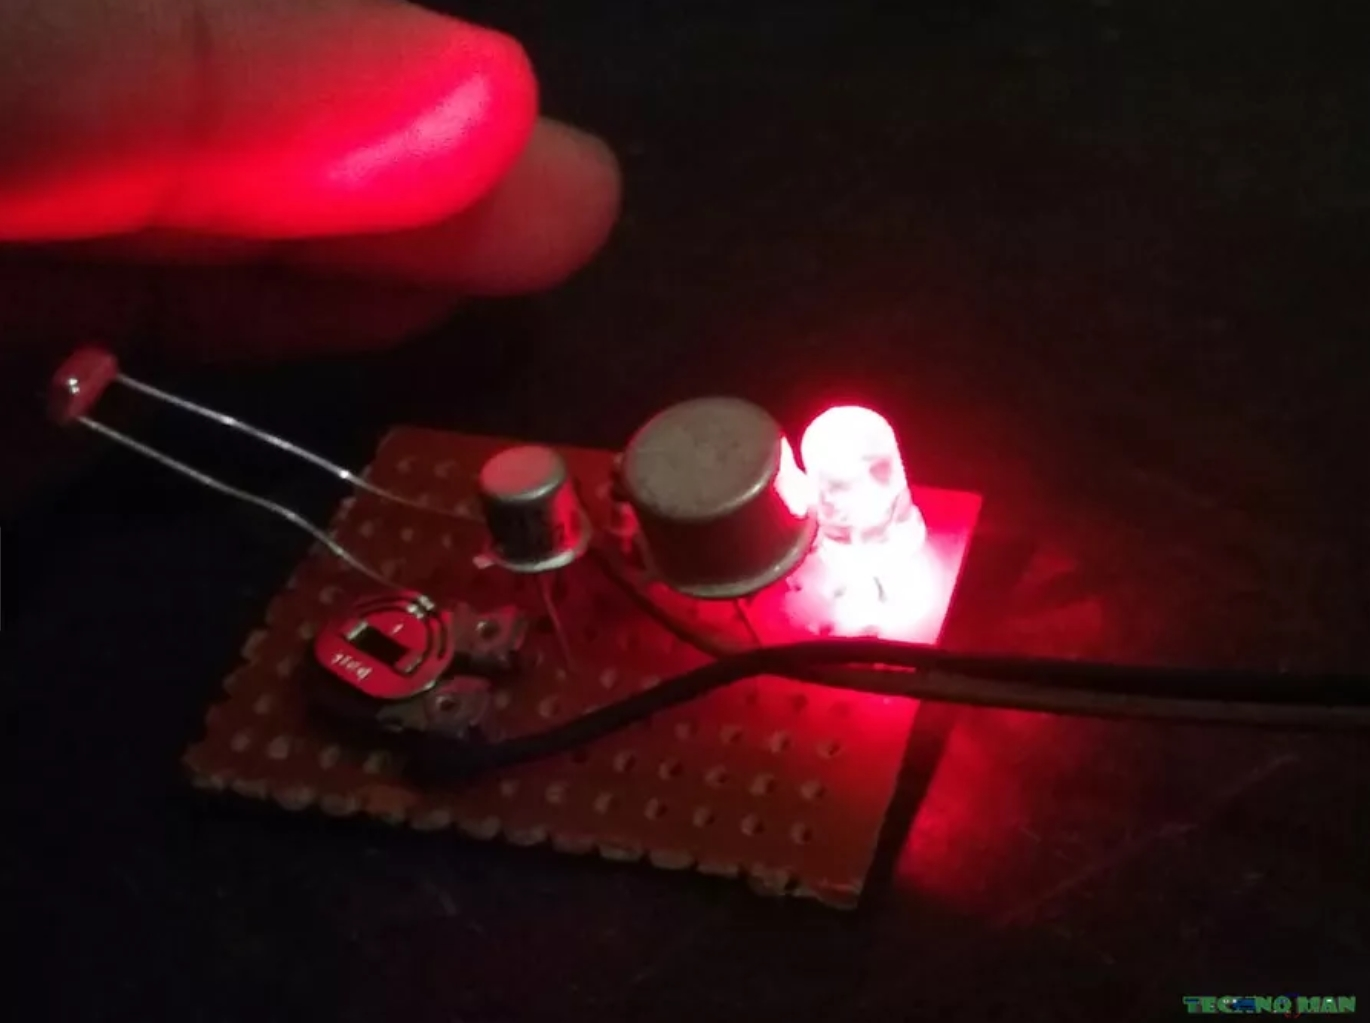
\includegraphics[scale=.75]{exp11-board}	
}

\section{Setup}
\label{sec-1}

First you will need to download, unzip, and install the Arduino Integrated Development Environment (IDE) from
\url{https://www.arduino.cc/en/Main/Donate} (does not need admin privileges).

\section{How it works}
\label{sec-2}
The automatic night light project is a LED light, powered by a battery, that is able to be automatically turned on in a dark environment. The most interesting part of the circuit is using light dependent resistor (LDR) that allows the circuit to behave in different lighting scenarios. The LDR changes the circuit and thus the corresponding LED depending on the amount of light it receives.

This project will be completed through soldering. Soldering is a method of creating a joint between electrical components. The most important part of soldering is creating a solid electrical connection between the electrical components. Solder is a type of alloy that usually comes rolled up like a wire. 

\centerline{
	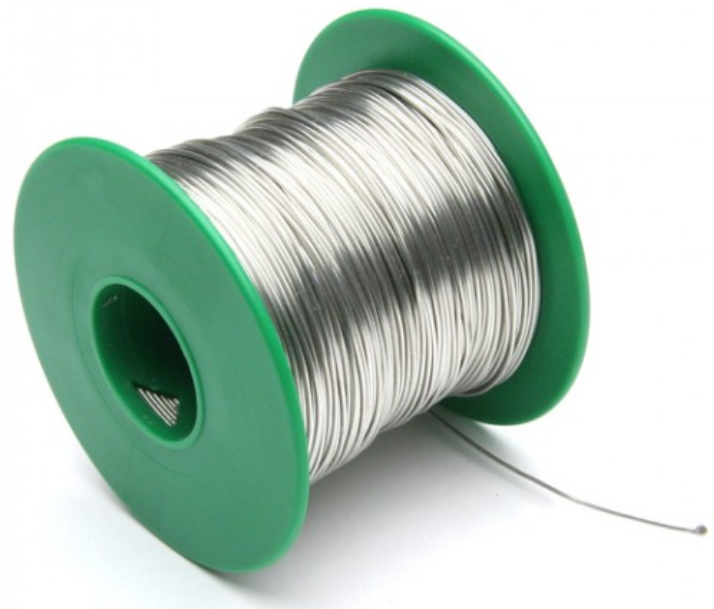
\includegraphics[scale=.75]{exp11-solder}	
}

Solder is used with a soldering iron in order to create the joint. The soldering iron is a hot piece of metal with a pointed tip that is able to melt the solder. The melted solder can then be used to make a connection from the electrical components you wish to connect. 

\centerline{
	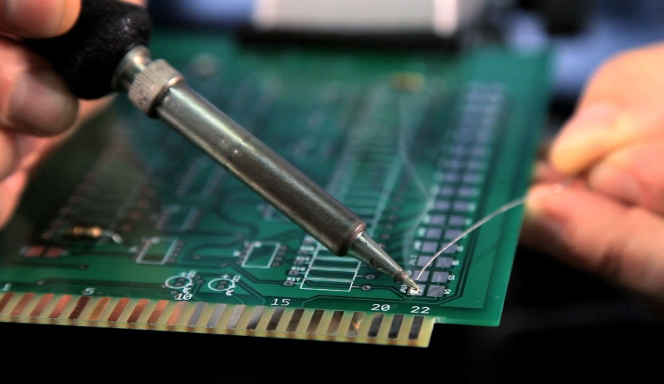
\includegraphics[scale=1.5]{exp11-iron}	
}
 
\section{Building The Circuit}
\label{sec-3}

The first step to successfully build and solder the circuit is to construct it on a electronic prototyping board called a perf board. A perf board is a board with through holes in it that allows electrical components to be set on prior to soldering. The board serves as a base that keeps the electrical components in place. Build onto the perf board with the schematics of the circuit shown below. 

\centerline{
	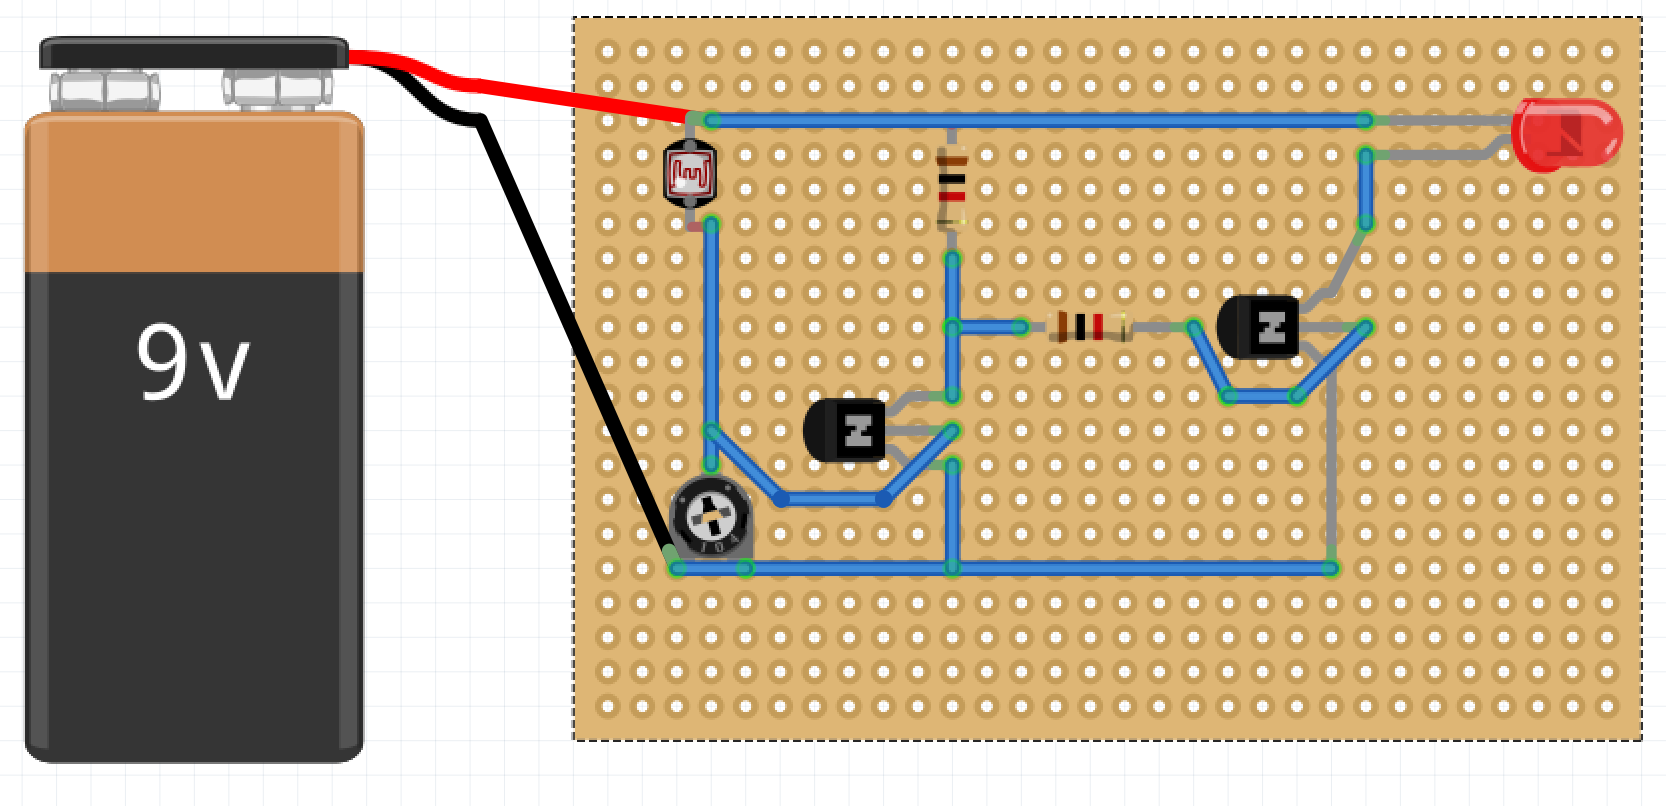
\includegraphics[scale=.75]{exp11-circuit}	
}

Once the components are correctly placed on the perf board, the next step is soldering. It is ideal to start solder at components that are in the middle of the circuit and might be hard to reach later. The first step in soldering is heating up the soldering iron to the desired temperature. The temperature has to be high enough to melt the solder. Once the soldering iron is hot enough, touch the solder to the tip of the iron and get a good amount of solder onto the iron. Taking the soldering iron with melted solder on it, you want to touch it to the two components you want to solder together. After a solder connection is made, a digital multimeter (DMM) can be used on the continuity setting to test the soldering connection. This will allow you to catch soldering problems early. The rest of the circuit can be soldered now but remember to solder hard to reach spots early. 

\section{Going Further}
\label{sec-6}
Once the circuit is accurately responding to the light, the project can be taken to the next step. 

\begin{itemize}
	\item If the LED is removable, try testing with different color LEDs.
	
	\item Build a custom container so that the electrical components are all hidden and the night light is easily portable. 
\end{itemize}

\end{document}

